\documentclass[en,hazy,blue,screen,14pt]{elegantnote}
\usepackage[T1]{fontenc}
\usepackage[latin9]{inputenc}
\usepackage{babel}
\usepackage{float}
\usepackage{textcomp}
\usepackage{amsmath,amsfonts,amssymb}
\usepackage{amsthm}
\usepackage{graphicx}
%\usepackage[ruled,vlined]{algorithm2e}
\PassOptionsToPackage{normalem}{ulem}
\usepackage{ulem}
\usepackage{mathtools}
\usepackage{url}
\usepackage{hyperref}
\usepackage{algorithm, algpseudocode}

\renewcommand\qedsymbol{$\blacksquare$}
\DeclarePairedDelimiter{\ceil}{\lceil}{\rceil}
\newcommand\tab[1][1cm]{\hspace*{#1}}
\newenvironment{claim}[1]{\par\noindent\underline{Claim:}\space#1}{}
\newenvironment{claimproof}[1]{\par\noindent\underline{Proof:}\space#1}{\hfill $\blacksquare$}
\renewcommand{\algorithmicrequire}{\textbf{Input:}}
\renewcommand{\algorithmicensure}{\textbf{Output:}}

\title{Class Notes\\CIS 502 Analysis of Algorithm\\5-Dynamics Programming}
\author{Da Kuang}
\institute{University of Pennsylvania}
% \version{1.00}
\date{}

\begin{document}

\maketitle
\newpage
% \input{}
\section{Introduction}
Dynamic programming is on the halfway of the continuum between brute-force algorithms and greedy algorithms. Brute-force is a strategy to use when you have no idea what to do. So you look at the problem and try every possible solution. Then see the best among the results. On the other extreme, greedy algorithm is used when you have a perfect sense what to do. So that you only need to do whatever looks cheapest to do now. By comparison, brute-force tries everything while greedy goes in a very directed way.

Interestingly, dynamic programming is a bit directed but is not that sure. Therefore, it breaks down the optimization problem into a series of decisions. For each decision, unlike greedy knowing the right thing to do, dynamic programming tries out every possible way within this decision. It is brute force locally but in a controlled so the algorithm not inefficient.

The performance of algorithm goes from greedy to dynamic programming then to brute force getting worse and worse. But the proofs is getting easier and easier. In brute force, you do not have to prove anything since it just simply tries everything and get the best answer. There is nothing clever that needs justification. Greedy algorithm, on the extreme, make a commitment to make a decision and we need to prove the decision is correct and we do not miss anything while only solving the local optimal.

\section{Learn Through Examples}
\subsection{Station Placement Problem}
Each town is located at a position weighted condition. Put down $K$ stations to minimize the maximum distance that a resident of any town has to commute to the nearest station.

\begin{figure}[H]
	\centering
	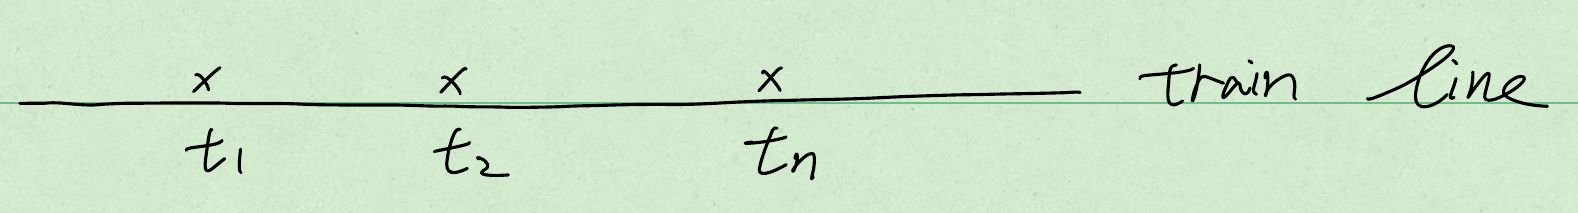
\includegraphics[width=0.5\textwidth]{fig/train-line.png}
\end{figure}

Greedy algorithm does not work for this problem. In greedy algorithm, unusually, we first find the set of town that must be served by the last station. Use greedy choice to identify that location and then recursively solve the problem. But we do not know how many town does the last station must serve and there is no obvious greedy strategy to answer this question.
 
Dynamic programming ask the same question, how many town should be served by the last station. But unlike greedy, since we do not know the answer, we try all the possible answers. 

Suppose the last station serves town $t_i, t_{i+1}, \cdots, t_n$ for some $i$. 

Notation: $C(n, k) = \text{cost of serving towns } t_1, \cdots, t_n$ with $k$ stations. Generally, $C(i, j)$ means the cost of serving towns $t_i, \cdots, t_j$ with $j$ station.

If someone told us that the optimal solution is for the last station to serve town $t_i^*, \cdots, t_n$, then 
\[C(n,k) = \max(\frac{t_n - t_i^*}{2}, ~C(i^* - 1, ~k - 1)).\]

Since we do not know $i$, we can write
\[C(n, k) = \min_{i = 1, \cdots, n}(\max(\frac{t_n - t_i}{2}, ~C(i -1, ~k - 1))).\]

Even though the number of sub-problems look like every big, there are actually only $n \times k$ kinds of problems.

\subsubsection{First algorithm}

Compute $C(n, k)$ exactly as in the recursion above.

\begin{algorithm}[H] 
	\caption{First Algorithm}
	\label{alg:loop}
	\begin{algorithmic}[1]
	\Require{n, k} \textbf{\textbf{}}
	\Ensure{Optimal Result}
	\Statex

%	\Comment{The g.c.d. of a and b}
	\Function{C}{$n,k$}
		\If {Base Cases}
			\State {$C(0, k \ge 0) = 0$}
			\State {$C(i, 1) = \frac{t_i - t_1}{2}$}
			\State {$C(i, i) = 0$}
		\Else
			\State {$min\_answer$ $\gets$ $\infty$}
			\For{$i \gets 1$ to $n$}      
			\If {$\max(\frac{t_n - t_i}{2},~C(i-1, k-1)) < min\_answer$}               
			\State {Update $min\_answer$}
			\EndIf
			\EndFor
			\State \Return {$min\_answer$}
		\EndIf
	\EndFunction
	\end{algorithmic}
\end{algorithm}

This recursive algorithm runs exponential time but we don't have too many distinct sub-problems. It is because we are solving the same sub-problems repeatedly.

Maintain solutions to solve sub-problems in a 2-D array. The C function, when called with argument $(i, j)$, first check if $C(i, j)$ is a known value in the array. If so, return it without any further call. So every sub-problem is solved only once. There are $n \times k$ sub-problems each take $O(n)$ time. It leads to a $O(n^2 k)$ algorithm.

Recall that we remember the answer of solved sub-problems and cutting short the recursion if the problem has been solved. This kind of techniques is called \textbf{memorization}.



\subsection{Check Binary Pattern}
Dynamic Programming(DP) is unusually used in Optimization problem such as the first example. But it could be used in other field as well. In this example, DP is used in a counting problem.

Given a number of $m$ in unary, count the number $n$ of binary string of length $m$ that do not contain the pattern $11$. For instance, in the following example, there are $5$ strings with length $3$ which does not containing $11$. 

\begin{figure}[H]
	\centering
	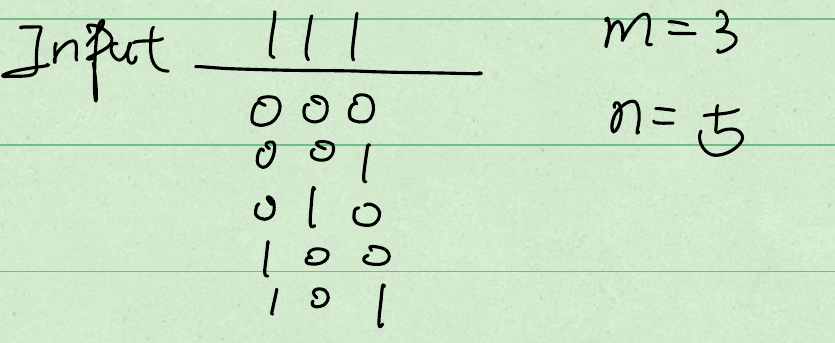
\includegraphics[width=0.3\textwidth]{fig/bin-pattern.png}
\end{figure}

\paragraph{Remark: why input is unary}The answer of the problem could be near $2^n$ string with $n$ bits long. If n is given by binary, your input is $\log n $ bits. In this case, even write down the answer would be an exponential time algorithm. Therefore, make the input unary reduce the size of the problem and make it solvable.

Say a string is valid if it does not contain the pattern ``$11$''.
\paragraph{Top Level Question:} 
\begin{itemize}
	\item Count the number of valid string of length $n$ ending in $0$.
	\item Count the number of valid string of length $n$ ending in $1$.
\end{itemize}

The valid strings of length $n$:
\begin{figure}[H]
	\centering
	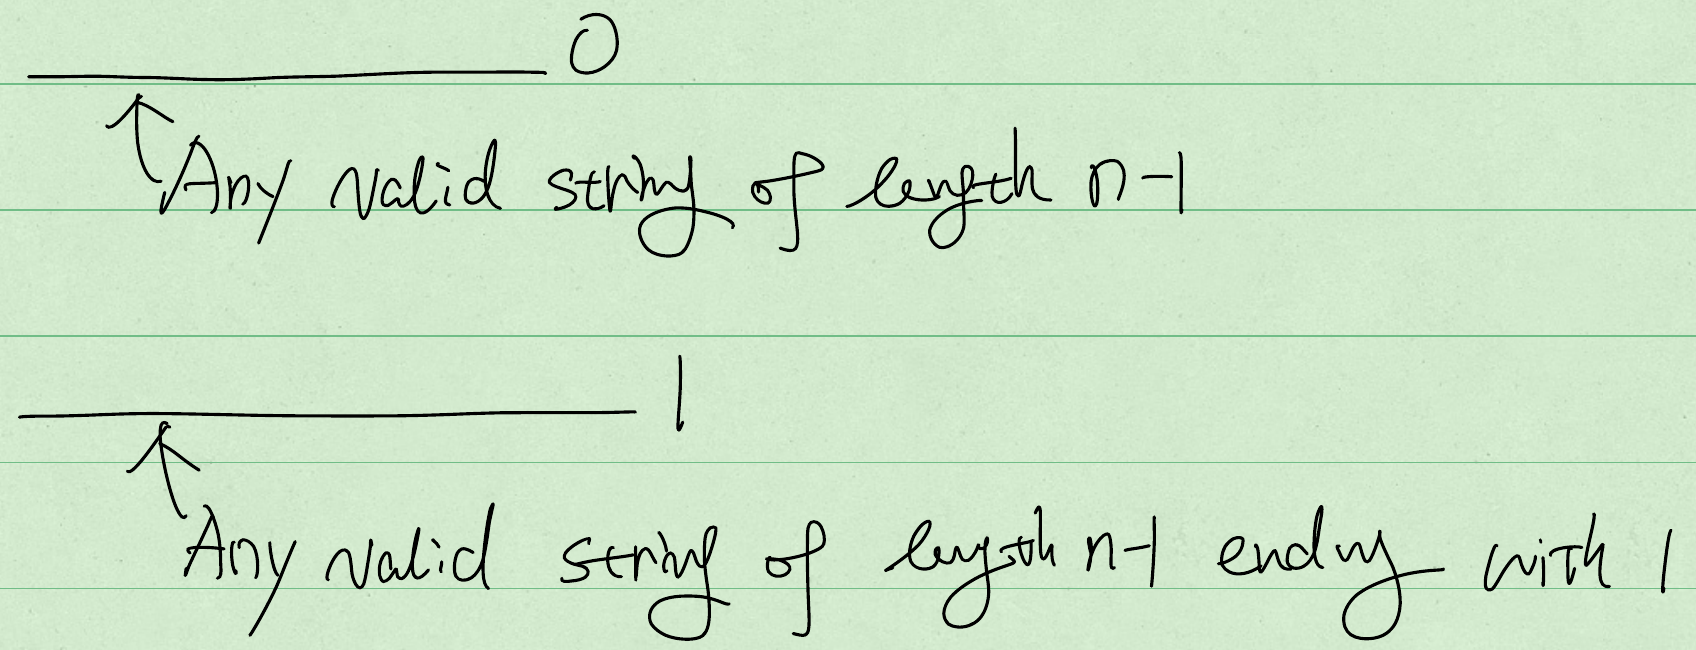
\includegraphics[width=0.5\textwidth]{fig/valid-str.png}
\end{figure}

Let make the following notation,
\begin{itemize}
	\item $S_1(n) = \#$ of valid string of length $n$, ending with $1$.
	\item $S_0(n) = \#$ of valid string of length $n$, ending with $0$.
\end{itemize}

So we have $S(n) = S_0(n) + S_1(n)$, where
\begin{align*}
	S_1(n) =& S_0(n-1)\\
	S_0(n) =& S(n-1) = S_0(n-1) + S(n-1) 
\end{align*}

Therefore, $S(n) = 2S_0(n - 1) + S_1(n - 1)$. In base cases, $S_1(1) = S_0(1) = 1$.



\subsection{Find Longest Acending Subsequence}
Given a sequence of positive integers, $a_1, a_2, \cdots, a_n$. A sub sequence is a sequence $ a_{i1}, a_{i2}, \cdots, a_{ik}$, where $i1 < i2 < \cdots < ik$. We say a subsequence $a_{i1}, a_{i2}, \cdots, a_{ik}$ is increasing if $a_{i1} < a_{i2} < \cdots < a_{ik}$.

For example, in the sequence
\[\{9, 5, 27, 2, 6, 1, 9, 8, 3, 1\},\]
$\{5, 6, 8, 11\}$ is an increasing subsequence.

\begin{lemma}
	In any sequence of length $n^2 + 1$, there is either an increasing sequence of length $n+1$ or decreasing sequence of length $n+1$.
\end{lemma}

\begin{proof}
	Let $a_1, a_2, \cdots, a_{n^2 + 1}$ be a sequence of $(n^2 + 1)$ distinct real numbers. Associate an ordered pair with each term of the sequence, namely, associate ($i_k$, $d_k$) to the term ak, where $i_k$ is the length of the longest increasing subsequence starting at $a_k$, and $d_k$ is the length of the longest decreasing subsequence starting at $a_k$.
	
	Suppose that there are no increasing or decreasing sub sequences of length $n+1$ or longer. Then $i_k$ and $d_k$ are both positive integers less than or equal to $n$, for $k = 1, 2, \cdots, n^2 + 1$. Hence, by the product rule there are $n^2$ possible ordered pairs for $(i_k, d_k)$. By the pigeonhole principle, two of these $n^2 + 1$ ordered pairs are equal.

	In other words, there exist terms $a_s$ and $a_t$, with $s < t$ such that $i_s = i_t$ and $d_s = d_t$. We will show that this is impossible. Because the terms of the sequence are distinct, either $a_s < a_t$ or $a_s > a_t$. 
	
	If $a_s < a_t$, then, because $i_s = i_t$, an increasing subsequence of length $i_t + 1$ can be built starting at as, by taking as followed
	by an increasing subsequence of length it beginning at at. This is a contradiction. 
	
	Similarly, if $a_s > a_t$, the same reasoning shows that ds must be greater than $d_t$, which is a contradiction.
\end{proof}

Dynamic Programming: Find the length of the longest sub sequence.

Top level question: Is $a_n$ in the longest increasing sequence? Unfortunately, this is not a good question, for example, for the sequence $100, 1, 2, 3, 4, 8$, suppose we answer "YES" to the top level quest "is 100 in the longest increasing sequence?". Then neither any follow-up number could be added into the longest sequence after 100. Therefore we need more information to carry over.

Actually, this problem takes some extra work comparing with the stander DP strategy.

$\text{Best}(i,l) = x$ if the increasing sequence of length $l$ in the prefix $a_1, \cdots, a_i$ with the smallest ending number ends in $x$.
For example, in sequence $100, 1, 2, 3, 4, 8$,
\begin{itemize}
	\item $\text{Best}(1,1) = 100$
	\item $\text{Best}(2,1) = 1$
	\item $\text{Best}(2,2) = +\infty$
\end{itemize}
One more example, $$5, 10, 7, 3, 8, 4, 9, 6$$
\begin{itemize}
	\item $\text{Best}(1,1) = 5$
	\item $\text{Best}(1,2) = +\infty$
\end{itemize}

Inductively assume that for some $i$, we have Best$(i, l)$ for all $l$.
When we see $a_{i+1}$, what would we do?

If $i = 4$,
\begin{itemize}
	\item $\text{Best}(4,1) = 3$
	\item $\text{Best}(4,2) = 7$
	\item otherwise, $+\infty$
\end{itemize}

If $i = 5$,
\begin{itemize}
	\item $\text{Best}(5,1) = 3$
	\item $\text{Best}(5,2) = 7$
	\item $\text{Best}(5,3) = 8$
	\item otherwise, $+\infty$
\end{itemize}

Here is the array of ends of best sequence of variants length update $a_i$. What you do with the new element is actually find the place where it will go. It can be done by binary search to find the place where the new element will go and make the new element replace the one after it. 

First of all, the array is sorted. The end of the best increasing sequence of length 1 is going to be less than the end of the best increasing sequence of length 2. It can be proved by contradiction. If some sequence of length 3 has a better ending than the sequence of length 2, you can take the first two elements from the sequence to have a better result than the current sequence of length 2.

So when a new element comes along, you binary search for it and wherever it want to go, we replace the next element by the new element.

The algorithm take one binary search for each new element so the total time is $T(n) = O(n\log n)$

This is a dynamic programming problem since we remember the result from what we have solved to get the best sequence for the a new element.




\subsection{All Pair Shortest Path}
\begin{itemize}
	\item Input: Weighted directed graph
	\item Goal: Compute a matrix of shortest path distances between every pair of vertices
\end{itemize}

The entry $D_{ij}$ of matrix $D$ is the distance of the shortest path from vertex $i$ to vertex $j$.

\subsubsection{Adjacency Matrix}
Adjacency Matrix is a representation of a weighted directed graph,

\[
	A[i, j]= 
		\begin{cases}
			w(i,j),& \text{if } (i, j)\in E\\
			\infty,              & \text{otherwise}
		\end{cases}
\]

What is the diagonal entries of $A$? They are all 0s.

What does $A^2$ mean?
\[
	A^2[i, j] = \sum_k A[i,k] \times A[k, j]
\]
Let's define a new matrix product for graph,

\[
	A^2[i, j] = \operatorname*{argmin}_k A[i,k] + A[k, j]
\]
\end{document}
